
\documentclass{article}

\usepackage[left=2cm,right=2cm, top=2cm, bottom = 2cm]{geometry}
\usepackage{amsfonts}

\usepackage{amsmath}
\usepackage{xcolor}

\usepackage{tikz}
\usepackage{subfigure}



\pagestyle{empty}

\setlength{\tabcolsep}{15pt}


\newcommand{\deriv}[3][]{\frac{\mathrm{d}^{#1}#2}{\mathrm{d}#3^{#1}}}
\newcommand{\diff}{\;\mathrm{d}}

\newcommand{\norm}[1]{\left|\kern-1pt\left|#1\right|\kern-1pt\right|}
\newcommand{\bra}[1]{\left\langle #1 \,\right|}
\newcommand{\ket}[1]{\left|\, #1\right\rangle}
\newcommand{\braket}[2]{\left\langle #1 \mid #2 \right\rangle}



\begin{document}

\title{Fourier Series}
\date{}

\maketitle
\thispagestyle{empty}



\Large

\textbf{\underline{Objective: To understand how a periodic function can be}}

\textbf{\underline{approximated by a series of trigonometric waves, or complex}}

\textbf{\underline{exponentials.}}






\vspace{5mm}



\textbf{Recap/Warm-up: Orthonormal Approximations:}\bigskip



Recall that $L_2([0,2\pi])$ is the vector space of square-integrable functions from $[0,2\pi]$ to $\mathbb{R}$, with the inner product defined by
\[\braket{f}{g}=\frac{1}{\pi}\int_0^{2\pi} f(x)g(x)\diff x.\]

Recall also that if $v_1,\hdots,v_n$ are orthogonal, then the best approximation to $v$ by a linear combination of $v_1,\hdots,v_n$ is
\[\sum_{i=1}^n \braket{v}{v_i}v_i.\]

 Let $f(x)=|x-\pi|-\frac{\pi}{2}$. Recall that $\sin(nx)$ and $\cos(nx)$ for positive integer $n$ are orthonormal.


\begin{enumerate}
	\item Show that
		\[\braket{f}{\sin(nx)} = 0.\]
	\item Show that
		\[\braket{f}{\cos(nx)} =\begin{cases} \frac{4}{\pi n^2}:& n=2k+1\\ 0: & n=2k.\end{cases}\]
	\item Hence write down $f_5(x)$, the best approximation to $f(x)$ by a linear combination of $\sin(x),\hdots,\sin(5x)$ and $\cos(x),\hdots,\cos(5x)$.
\end{enumerate}

\begin{center}
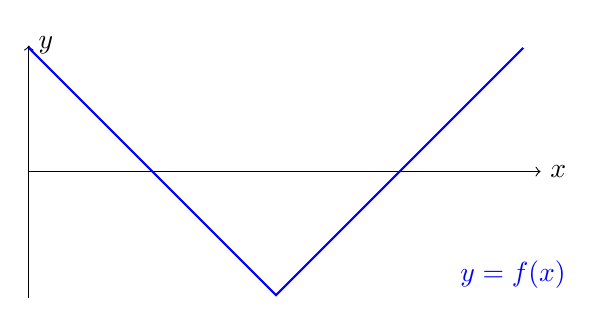
\begin{tikzpicture}
	\draw[->] (0,0) -- (6.5,0);
	\node[right] at (6.5,0) {$x$};
	\draw[->] (0,-1.6) -- (0,1.6);
	\node[right] at (0,1.6) {$y$};
	
	\draw[thick,blue] (0,1.57) -- (3.14,-1.57) -- (6.28,1.57);
	
	\node[blue,above left] at (current bounding box.south east) {$y=f(x)$};
\end{tikzpicture}
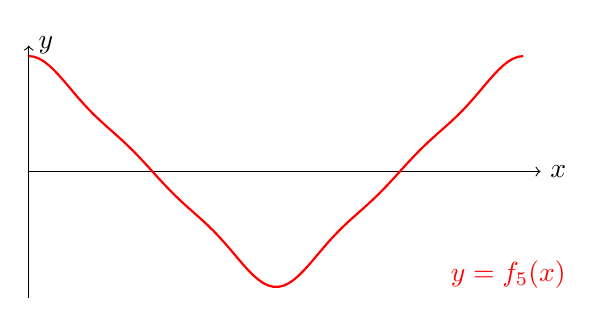
\begin{tikzpicture}
	\draw[->] (0,0) -- (6.5,0);
	\node[right] at (6.5,0) {$x$};
	\draw[->] (0,-1.6) -- (0,1.6);
	\node[right] at (0,1.6) {$y$};
	
	\draw[thick,red,domain=0:6.28,samples=100] plot (\x, { (4/3.14)*cos(\x r) + (4/(3.14*9))*cos(3*\x r) + (4/(3.14*25))*cos(5*\x r) });
	
	\node[red,above left] at (current bounding box.south east) {$y=f_5(x)$};
\end{tikzpicture}
\end{center}






\clearpage















\textbf{Theory: Fourier Series:}

\bigskip



We have seen that the functions $\sin(nx)$ and $\cos(nx)$ are orthonormal in $L_2([0,2\pi])$. Also, the constant function $\frac{1}{2}$ is a unit vector, and orthogonal to each of the sines and cosines. Therefore we have an infinite orthonormal family
\[\frac{1}{2},\sin(x),\cos(x),\sin(2x),\cos(2x),\hdots\]
Therefore, by the theory of orthonormal approximations, given any function $f$ in $L_2([0,2\pi])$, we can approximate $f$ by the first $N$ of these functions:
\[f(x)\approx f_N(x)=\frac{a_0}{2}+\sum_{n=1}^N \left[a_n\cos(nx)+b_n\sin(nx)\right],\]
where
\begin{align*}
	a_n&=\braket{f}{\cos(nx)}=\frac{1}{\pi}\int_0^{2\pi} f(x)\cos(nx)\diff x\\
	b_n &= \braket{f}{\sin(nx)}=\frac{1}{\pi}\int_0^{2\pi} f(x)\sin(nx)\diff x.
\end{align*}

We can take $N$ as large as we like; ignoring for the moment issues of convergence, we take the limit as $N$ tends to infinity and define the \textbf{Fourier series} of $f$ to be
\[\tilde{f}=\frac{a_0}{2}+\sum_{n=1}^\infty \left[a_n\cos(nx) + b_n\sin(nx)\right].\]

We will discuss convergence later.\medskip

So far we have only worked over the interval $[0,2\pi]$; however, there is nothing special about this interval. Given any interval of length $L$, $[a,a+L]$, we can define an inner product on $L_2([a,a+L])$ by
\[\braket{f}{g}=\frac{2}{L}\int_a^{a+L}\!\!\! f(x)g(x)\diff x,\]
and then the Fourier series of a function $f$ over $[a,a+L]$ is
\[\tilde{f}=\frac{a_0}{2}+\sum_{n=1}^\infty \left[a_n\cos\left(\frac{2\pi nx}{L}\right) + b_n\sin\left(\frac{2\pi nx}{L}\right)\right],\]
where
\begin{align*}
	a_n&=\braket{f}{\cos\left(\frac{2\pi nx}{L}\right)}=\frac{2}{L}\int_a^{a+L}\!\!\! f(x)\cos\left(\frac{2\pi nx}{L}\right)\diff x\\
	b_n &= \braket{f}{\sin\left(\frac{2\pi nx}{L}\right)}=\frac{2}{L}\int_a^{a+L}\!\!\! f(x)\sin\left(\frac{2\pi nx}{L}\right)\diff x.
\end{align*}



\clearpage





\textbf{Theory: Exponential Fourier Series:}

\bigskip


By Euler's Equation
\[e^{ix}=\cos(x)+i\sin(x),\]
we get the equations
\[\cos(x)=\frac{e^{ix}+e^{-ix}}{2},\qquad \sin(x)=\frac{e^{ix}-e^{-ix}}{2i}.\]

Using these, we can rewrite a Fourier series as a sum of exponentials; however, to do this, we must allow negative values of $n$, so our sum goes from $-\infty$ to $\infty$. Given a Fourier series
\[\tilde{f}(x)=\frac{a_0}{2}+\sum_{n=1}^\infty \left[a_n\cos\left(nx\right) + b_n\sin\left(nx\right)\right],\]
we substitute our above identities, and set $b_0=0$:
\begin{align*}
	F(t) &= \frac{a_0}{2} - \frac{b_0i}{2} + \sum_{n=1}^\infty \left[a_n\frac{e^{inx}+e^{-inx}}{2} + b_n\frac{e^{inx}-e^{-inx}}{2i}\right]\\
	&= \frac{a_0-b_0i}{2} + \sum_{n=1}^\infty \frac{a_n-b_ni}{2}e^{inx} + \sum_{n=1}^\infty \frac{a_n+b_ni}{2}e^{-inx}
\end{align*}

Since we have negative powers of $e$ occuring, it makes sense to allow $n$ to take negative values; how do our Fourier coefficients behave with negative values of $n$? We see that, simply substituting $-n$ into the definition:
\[a_{-n} = \frac{1}{\pi}\int_0^{2\pi} f(x)\cos\left(-nx\right)\diff x=a_n\]
since cosine is an even function. For the sine coefficients, on the other hand:
\[b_{-n} = \frac{1}{\pi}\int_0^{2\pi} f(x)\sin\left(-nx\right)\diff x=-b_n\]
since sine is an odd function. So we can extend our definition of the Fourier coefficients to negative values of $n$, with the simple relations $a_{-n}=a_n$, and $b_{-n}=-b_n$.

Therefore, in the second infinite series of our rearranged Fourier series above, we can write
\begin{align*}
	\sum_{n=1}^\infty \frac{a_n+b_ni}{2}e^{-inx}&=\sum_{n=1}^\infty \frac{a_{-n}-b_{-n}i}{2}e^{-inx}\\
	&= \sum_{n=-\infty}^1 \frac{a_n-b_ni}{2}e^{inx}.
\end{align*}
This makes the summands equal to those of the first infinite series, but the limits now go from $-\infty$ to $1$, instead of $1$ to $\infty$. The constant term also has the same form, so we can treat it as
\[\frac{a_n-b_ni}{2}e^{inx}\]
when $n=0$. Therefore every term we are adding has the same form, so we can combine them all into a single infinite sum:
\[\tilde{f}(x)=\sum_{n=-\infty}^\infty \frac{a_n-b_ni}{2}e^{inx}.\]\medskip


Now consider the coefficients in the above series. From the definitions, we have
\begin{align*}
	\frac{a_n-b_ni}{2} &= \frac{1}{2}\left[\frac{1}{\pi}\int_0^{2\pi}\!\!f(x)\cos\left(nx\right)\diff x -\frac{i}{\pi}\int_0^{2\pi}\!\! f(x)\sin\left(nx\right)\diff x\right]\\
	&=\frac{1}{2\pi}\int_0^{2\pi}\!\!f(x)\left[\cos\left(nx\right) - i \sin\left(nx\right)\right]\diff x\\
	&=\frac{1}{2\pi}\int_0^{2\pi}\!\! f(x)e^{-inx}\diff x.
\end{align*}

So we define
\[c_n=\frac{1}{2\pi}\int_0^{2\pi}\!\!f(x)e^{-inx}\diff x,\]
and write the \textbf{exponential Fourier series} of $f$ over $[0,2\pi]$ as
\[\tilde{f}(x)=\sum_{n=-\infty}^\infty c_n e^{inx}.\]\bigskip

As before, there is nothing special about the interval $[0,2\pi]$, we have simply used that for convenience. Over a general interval $[a,a+L]$, we let
\[c_n=\frac{1}{L}\int_a^{a+L}\!\!\!f(x)e^{-2\pi i nx/L}\diff x,\]
and then the Fourier series is
\[\tilde{f}(x) = \sum_{n=-\infty}^\infty c_ne^{2\pi inx/L}.\]




\clearpage



\textbf{Complex $L_2$-Space and Complex Inner Products:}\bigskip


So far we have focused on \textit{real-valued} square-integrable functions from $[0,2\pi]$ to $\mathbb{R}$. Even though complex numbers appear in the exponential form of the Fourier series, if the original function $f$ was real-valued, then the Fourier series will be too---the terms will appear in complex conjugate pairs, so the imaginary parts will cancel out. However, there is no problem with starting with a complex-valued square-integrable function.

Indeed, we can define a complex inner-product on the space of complex-valued square integrable functions on $[0,2\pi]$ by
\[\braket{f}{g}=\frac{1}{2\pi}\int_0^{2\pi} f(x)\overline{g(x)}\diff x,\]
where the bar denotes complex conjugate. Then we could check that the functions $e^{inx}$ are orthonormal for all integer values of $n$ (positive and negative), and hence the best approximation to $f$ by these orthonormal functions (ignoring issues of convergence) is given by
\[\sum_{n=-\infty}^\infty \braket{f}{e^{inx}}e^{inx}.\]
But
\[\braket{f}{e^{inx}}=\frac{1}{2\pi}\int_0^{2\pi} f(x)e^{-inx}\diff x=c_n,\]
so this is exactly the exponential form of the Fourier series.\bigskip

We could have developed the theory in terms of complex-valued functions right from the start, but for simplicity we stuck to real-valued functions. However, from now on, $L_2([0,2\pi])$ will refer to the vector space of \textit{complex-valued} square-integrable functions on $[0,2\pi]$, with the inner product defined above.







\clearpage



\textbf{Convergence:}\bigskip


We know that we can approximate any function in $L_2([0,2\pi])$ with sines and cosines, and that the error in this approximation will get smaller the more terms we take, but how small does the error get? Can we get an arbitrarily good approximation, or is there some lower bound on the error, and no matter how many terms of the Fourier series we take, we can never get a better approximation than some amount?

It can be proved that we can make the error as close to zero as we like by taking enough terms in the Fourier series; \textit{i.e.}, that the Fourier series does actually converge to the original function (with respect to the $L_2$-metric). This proof is difficult, so we defer it to later; for now, let's just make some observations that will allow us to check that specific Fourier series converge to the desired function.

Recall that on the last sheet we used induction to prove that if $v$ is approximated by $\sum \lambda_iv_i$, then the square of the error is given by
\begin{equation}
	\norm{v-\sum_{i=1}^n \lambda_iv_i}^2=\norm{v}^2 - 2 \sum_{i=1}^n \lambda_i\braket{v}{v_i} + \sum_{i=1}^n \lambda_i^2 .\tag{$\star$}
\end{equation}
This was the key equation we used to show that taking $\lambda_i=\braket{v}{v_i}$ minimises the error. So when taking this best approximation, the square of the error in the approximation is
\[\norm{v-\sum_{i=1}^n \lambda_iv_i}^2=\norm{v}^2 - \sum_{i=1}^n \braket{v}{v_i}^2.\]

Now, if $f$ is a function in $L_2([0,2\pi])$, then the functions $e^{inx}$ for $n=0,1,-1,2,-2,\hdots$ are orthonormal, and if we approximate $f$ by $e^{inx}$ for $i$ from $-N$ to $N$ (\textit{i.e.}, the first $2N+1$ terms of the exponential Fourier series), then the squared error is
\[\norm{f-\sum_{n=-N}^N c_n e^{inx}}^2=\norm{f}^2 - \sum_{n=-N}^N c_n^2.\]

So for any particular function $f$, once we have computed the Fourier coefficients $c_n$, if we can prove that the sum of the coefficients converges to $\norm{f}$, then the error in the Fourier approximation converges to 0, so the Fourier series is distance 0 from the original function in the $L_2$-metric; this implies that it is the same as the original function almost everywhere. Note, however, that at a ``small'' set of points (\textit{e.g.}, any countable set), the Fourier series could disagree with the original function. For instance, if the original function is piecewise-continuous, the Fourier series will not necessarily converge to the correct value at the discontinuities.

\clearpage


\textbf{Example:}\bigskip


We saw in the warmup that for $f(x)=|x-\pi|-\frac{\pi}{2}$, the Fourier coefficients are
\[a_n=\begin{cases} \frac{4}{\pi n^2}:&n=2k+1\\ 0: & n=2k\end{cases}\]
and $b_n=0$. Therefore the exponential coefficients $c_n=\frac{1}{2}(a_n-b_ni)$ are given by
\[c_n=\begin{cases} \frac{2}{\pi n^2}:& n=2k+1\\ 0: & n=2k.\end{cases}\]
Therefore the exponential Fourier series of $f$ is
\[\tilde{f}(x)=\sum_{n=-\infty}^{\infty} \frac{2}{\pi (2n+1)^2}e^{(2n+1)ix}\]
and the squared error from taking the sum from $-N$ to $N$ is
\[\norm{f-\sum_{n=-N}^N \frac{2}{\pi (2n+1)^2}e^{(2n+1)ix}}^2=\norm{f}^2-\sum_{n=-N}^N \frac{4}{\pi^2 (2n+1)^4}.\]

First we compute $\norm{f}^2=\frac{\pi^2}{12}$. So we wish to show that
\[\sum_{n=-\infty}^\infty \frac{4}{\pi^2(2n+1)^4}=\frac{\pi^2}{12}.\]
Rearranging, we wish to show that
\[3\sum_{n=-\infty}^\infty (2n+1)^{-4}=\left(\frac{\pi}{2}\right)^4.\]

The terms for negative $n$ are precisely the terms for positive $n$, just shifted; since $(2(-n)+1)^{-4}=(-2n+1)^{-4}=(2n-1)^{-4}$, so we can rewrite the left-hand side as
\[6\sum_{n=0}^\infty (2n+1)^{-4}.\]


Note that if we sketch the graph of $y=(2x+1)^{-4}$ and approximate the area under the graph for $k\leq x<\infty$ by drawing rectangles for each integer $n> k$ of height $(2n+1)^{-4}$, and width from $n-1$ to $n$, then we must be underestimating the area. Therefore
\begin{align*}
	6\sum_{n=k+1}^\infty (2n+1)^{-4}&\leq 6\int_k^\infty (2x+1)^{-4}\diff x\\
	&=\left[-(2x+1)^{-3}\right]_k^\infty\\
	&= (2k+1)^{-3}.
\end{align*}


Moreover, since each term in the sum is positive, the sum only increases as we add more terms. Therefore
\[6\sum_{n=0}^\infty (2n+1)^{-4}-(2k+1)^{-3}\leq 6\sum_{n=0}^{k-1}(2n+1)^{-4}\leq 6\sum_{n=0}^\infty (2n+1)^{-4}.\]
In words, if we sum the first $k-1$ terms of the series, we underestimate the total value of the sum by at most $(2k+1)^{-3}$.

Firstly, this proves that the series converges, and secondly it allows us to estimate its value to any desired precision. Suppose we want to compute the sum to an accuracy of 8 decimal places; if we can get the error smaller than $10^{-9}$, this will certainly guarantee that; so we want to find $k$ such that $(2k+1)^{-3}\leq 10^{-9}$. Taking cube roots, we want $(2k+1)^{-1}\leq 10^{-3}$, so $2k+1\geq 1000$, so $k\geq\frac{999}{2}$. So if we sum the first $500$ terms of the series, we should get the correct value for the infinite series to within 8 decimal places.

With a short bit of Python code, we find that
\[6\sum_{n=0}^{500} (2n+1)^{-4} \approx 6.088068188631126;\]
whereas $\left(\frac{\pi}{2}\right)^4\approx 6.088068189625151$. We see that these agree to 9 decimal places, and we know that the first value is the correct value of the sum to 8 decimal places. Therefore the squared error in the Fourier series,
\[\norm{f-\sum_{n=-N}^N \frac{2}{\pi (2n+1)^2}e^{(2n+1)ix}}^2=\norm{f}^2-\sum_{n=-N}^N \frac{4}{\pi^2 (2n+1)^4},\]
is 0 to at least 8 decimal places. Taking square roots, the error $\norm{f-\tilde{f}}$ is 0 to at least 4 decimal places.\bigskip


Although we haven't proved that the error can be made arbitrarily small, we can certainly believe that it looks likely, and we have a simple procedure for checking it to any desired level of precision.






\clearpage




{\bf Key Points to Remember:}

\vspace{5mm}

\begin{enumerate}
	\item The Fourier series of $f$ is
		\[\tilde{f}=\frac{a_0}{2}+\sum_{n=1}^\infty \left[a_n\cos\left(\frac{2\pi nx}{L}\right) + b_n\sin\left(\frac{2\pi nx}{L}\right)\right],\]
		where
		\begin{align*}
			a_n&=\braket{f}{\cos\left(\frac{2\pi nx}{L}\right)}=\frac{2}{L}\int_a^{a+L}\!\!\! f(x)\cos\left(\frac{2\pi nx}{L}\right)\diff x\\
			b_n &= \braket{f}{\sin\left(\frac{2\pi nx}{L}\right)}=\frac{2}{L}\int_a^{a+L}\!\!\! f(x)\sin\left(\frac{2\pi nx}{L}\right)\diff x.
		\end{align*}
	\item The sum of the first $N$ terms of the Fourier series is the best approximation to $f$ by a linear combination of the orthonormal functions
		\[\frac{1}{L},\sin\left(\frac{2\pi x}{L}\right),\cos\left(\frac{2\pi x}{L}\right),\hdots,\sin\left(\frac{2\pi Nx}{L}\right),\cos\left(\frac{2\pi Nx}{L}\right).\]
	\item The \textbf{exponential form} of the Fourier series is
		\[\tilde{f}=\sum_{n=-\infty}^\infty c_ne^{2\pi inx/L},\]
		where
		\[c_n=\frac{a_n-b_ni}{2}=\frac{1}{L}\int_a^{a+L}\!\!f(x)e^{-2\pi inx/L}.\]
	\item For any function in an $L_2$-space, the Fourier series converges to that function almost everywhere; the proof is hard, but we can look at it if you like.
	\item Even without proving convergence in general, for any particular function $f$, the squared error in the approximation by the Fourier series (with respect to the $L_2$-metric) is given by
		\[\norm{f-\tilde{f}}^2=\norm{f}^2-\sum_{n=-\infty}^\infty c_n^2.\]
		Therefore if we can show that the sum of the squared Fourier coefficients converges to $\norm{f}$, then we know that the Fourier series converges to the original function. Though this is often difficult to prove in practice, error bounds can often be obtained.
\end{enumerate}









\end{document}